\section{Réseaux de neurones profonds}\label{chapter-ML-section-DNN}
Les réseaux de neurones (NN, \emph{Neural Networks}) sont un autre type de modèle permettant d'approximer la fonction reliant les entrées $\set{\vec{x}_i}$ aux cibles $\set{\ytruei}$~\cite{DNN}.
La section~\ref{chapter-ML-section-DNN-neuron} introduit le concept de neurone dans le cadre du ML.
Puis, les réseaux de neurones sont présentés dans la section~\ref{chapter-ML-section-DNN-networks}.
L'entraînement de ce type de modèle est discuté section~\ref{chapter-ML-section-DNN-training}.
\subsection{Neurones}\label{chapter-ML-section-DNN-neuron}

\begin{figure}[h]
\centering
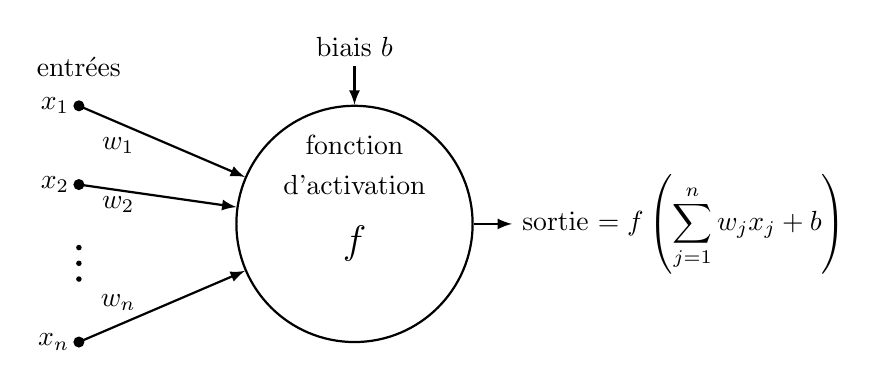
\begin{tikzpicture}

\node [draw, thick, circle, minimum size = 3 cm] (N) at (0,0) {};

\foreach \yi/\N in {1.5/1,0.5/2,-1.5/n}{
\fill (-3.5,\yi) circle(2pt) node [left] {$x_{\N}$};
\draw [thick, -latex] (-3.5,\yi) -- (N);
}

\draw (-3.5,1.75) node [above] {entrées};

\draw (-3,1) node {$w_1$};
\draw (-3,0.25) node {$w_2$};
\draw (-3,-1) node {$w_n$};

\foreach \x/\y in {-3.5/-.5}{
\fill (\x,\y) circle (1pt);
\fill (\x,\y+.2) circle (1pt);
\fill (\x,\y-.2) circle (1pt);
}

\draw [thick, latex-] (N) -- (0,2) node [above] {biais $b$};

\draw [thick, -latex] (N) -- (2,0) node (output) [right] {sortie $\displaystyle = f\left(\sum_{j=1}^n w_jx_j + b\right)$};

\draw (0,-.25) node {\Large $f$};
\draw (0,1) node {fonction};
\draw (0,.5) node {d'activation};

\end{tikzpicture}

\caption[Structure d'un neurone.]{Structure d'un neurone. Une fonction $f$ dite d'\og activation \fg{} est appliquée à la somme des entrées $x_i$ pondérées par les poids $w_i$ et du biais $b$ afin d'obtenir la valeur de sortie.}
\label{fig-chapter-ML-section-DNN-neuron-neuron_structure}
\end{figure}



Activation functions:
tanh, sigmoïd mostly for classification,
linear, relu, elu, selu, softmax, softplus ...
\subsection{Réseaux de neurones}\label{chapter-ML-section-DNN-networks}


\begin{figure}[h]
\centering
\def\drawN{}
\renewcommand{\drawN}[2][c]{
\node [draw, circle, minimum size = .66 cm] (#1) at (#2) {};
}
\def\linkN#1#2{
\draw [-latex] (#1) -- (#2);
}
\def\yscale{1.25/1.75}
\begin{tikzpicture}[scale=1.75]

\foreach \y in {0,1,2,-2}{
\foreach \x in {1,2,...,5}{
\drawN[\x\y]{\x,{\y*\yscale}}
}
}

\foreach \yi/\N in {1.5/1,0.5/2,-1.5/n}{
\fill (-.5,{\yi*\yscale}) circle(2pt) node [left] {$x_{\N}$};
\foreach \y in {0,1,2,-2}{
\draw [-latex] (-.5,{\yi*\yscale}) -- (1\y);
}
}

\drawN[No]{6.5,0}

\draw [-latex] (No) --+ (.5,0) node [right] {$y=F(\vec{x})$};

\foreach \ya in {0,1,2,-2}{
\foreach \yb in {0,1,2,-2}{
\linkN{5\ya}{No}
\foreach \xa/\xb in {1/2,2/3,3/4,4/5}{
\linkN{\xa\ya}{\xb\yb}
}
}
}

\fill[white] (2.33,{-2.5*\yscale}) rectangle (4.66,{2.5*\yscale});

\foreach \x/\y in {-.5/-.5,1/-1,2/-1,5/-1}{
\fill (\x,{\y*\yscale}) circle (1pt);
\fill (\x,{(\y+.2)*\yscale}) circle (1pt);
\fill (\x,{(\y-.2)*\yscale}) circle (1pt);
}

\foreach \y in {0,1,2,-2}{
\fill (3.5,{\y*\yscale}) circle (1pt);
\fill (3.5+.2,{\y*\yscale}) circle (1pt);
\fill (3.5-.2,{\y*\yscale}) circle (1pt);
}

\foreach \x in {.25,5.75}{
\draw [thick, dotted, ltcolorblue] (\x,{-2.5*\yscale}) -- (\x,{2.5*\yscale});
}

\draw [ltcolorblue, left] (.25, {2.5*\yscale}) node {Couche d'entrée\vphantom{Àq}};
\draw [ltcolorblue] (3, {2.5*\yscale}) node {Couches cachées\vphantom{Àq}};
\draw [ltcolorblue, right] (5.75, {2.5*\yscale}) node {Couche de sortie\vphantom{Àq}};

\draw [thick, ltcolorred, latex-latex] (.25,{-2.5*\yscale}) -- (5.75,{-2.5*\yscale});
\draw [ltcolorred] (3, {-2.25*\yscale}) node {$N_L$\vphantom{Àq}};

\draw [thick, ltcolorred, latex-latex] (4.5,{-2.125*\yscale}) -- (4.5,{2.125*\yscale});
\draw [ltcolorred] (4.5, {0*\yscale}) node [left] {$N_N$\vphantom{Àq}};

\end{tikzpicture}

\caption[Structure d'un réseau de neurones.]{Structure d'un réseau de neurones. Une couche d'entrée comporte autant de neurones que de variables $x_i$. La couche de sortie en comporte autant que de valeurs à donner, \ie\ une. Les fonctions d'activation de ces deux couches sont linéaires. Entre elles se trouvent $N_L$ couches cachées, chacune contenant $N_N$ neurones. Diverses fonctions d'activation peuvent être utilisées dans les couches cachées.}
\end{figure}
\subsection{Entraînement}\label{chapter-ML-section-DNN-training}
L'entraînement d'un NN est le réglage des paramètres des neurones du réseau situés sur les couches cachées et la couche de sortie.
Il s'agit des poids $w_i$ et du biais $b$.
Pour un DNN avec
$n_\text{in} = \num{27}$ variables d'entrée,
$\NLayers = \num{3}$ couches cachées
de $\NNeurons = \num{1000}$ neurones,
le nombre de paramètres est ainsi de
\begin{align}
N_\text{params.}
&= \underbrace{\NNeurons \times (n_\text{in} + 1)}_\text{couche cachée 1} \!\!\!&\!\!\!+\,\,\,& \underbrace{(\NLayers -1)\times \NNeurons \times(\NNeurons+1)}_\text{autres couches cachées} \!\!\!&\!\!\!+\,\,\,& \underbrace{\NNeurons +1\vphantom{()}}_\text{couche de sortie}
\nonumber\\&
=
\num{28000} \!\!\!&\!\!\!+\,\,\,& 2\times\num{1001000} \!\!\!&\!\!\!+\,\,\,& \num{1001}
=
\num{2031001}
\mend[,]
\end{align}
soit près de deux millions.
Les termes \og $+1$ \fg{} correspondent aux biais $b$ à ajouter au nombre d'entrées des neurones.
\subsubsection{Initiation des paramètres}
Les biais $b$ sont initialement fixés à 0,
les poids $w_i$ à une valeur constante donnée ou aléatoirement selon une loi de probabilité.
Le mode d'initiation est un hyper-paramètre du modèle.
Lors de ces travaux, nous avons testé les lois normale et uniforme.
Dans le cas des DNNs, ces modes d'initiation peuvent être améliorés par la méthode de \citeauthor{glorot}~\cite{glorot} afin de faciliter l'entraînement.
Il s'agit alors des lois \og Glorot uniforme \fg{} et \og Glorot normale \fg, également testées.
\subsubsection{Fonction de coût et optimisation des paramètres}
La modification des paramètres du NN pourrait être réalisée \todo{ainsi} pour chaque événement du jeu de données d'entraînement.
Or, la nature des données à analyser peut mener à une stagnation, si deux événements donnent modifications opposées.
Afin d'éviter ce phénomène, la mise à jour des paramètres se fait à partir de \og mini-lots \fg, introduits section~\ref{chapter-ML-section-DNN-training-minibatch}.
Des algorithmes d'optimisation, adaptés aux mini-lots et dérivés du \emph{Gradient Descent}, sont présentés section~\ref{chapter-ML-section-DNN-training-optimizers}.
\subsubsection{Mini-lots et époques}\label{chapter-ML-section-DNN-training-minibatch}
Un mini-lot est un sous-ensemble du jeu de données.
L'entraînement se base alors sur la moyenne du gradient de la fonction de coût sur le mini-lot, au lieu de la valeur de ce gradient pour chaque événement.
\par
Une \og époque \fg{} de l'entraînement correspond à une utilisation de tous les mini-lots, \ie\ de tous les événements du jeu de données, pour modifier les paramètres du NN.
Le nombre maximal d'époques autorisé est de \num{500}, avec un arrêt prématuré au bout de \num{20} époques sans diminution de l'erreur absolue moyenne sur les données de validation.
\par
Pour ne pas biaiser l'entraînement à cause de l'ordre du jeu de données,
il est mélangé aléatoirement à chaque nouvelle époque.
La composition des mini-lots est donc également aléatoire.
La taille des mini-lots est fixée à $2^{11}=\num{2048}$ événements.
Une taille de la forme $2^n$ permet d'optimiser l'utilisation des GPUs (\emph{Graphics Processing Unit}) sur lesquels l'entraînement se fait~\cite{DNN}.
Les points de masse générés étant les entiers entre \num{50} et \SI{800}{\GeV}, soit \num{750} points de masse,
\num{2048} événements pris au hasard est un compromis entre
un petit mini-lot
et
une bonne probabilité de couvrir une large gamme de masse au sein d'un mini-lot.
\subsubsection{Algorithmes d'optimisation}\label{chapter-ML-section-DNN-training-optimizers}
Plusieurs algorithmes d'optimisation existent~\cite{DNN}, présentés de manière non exhaustive ci-après.
Le premier, SGD, est l'adaptation directe du \emph{Gradient Descent} aux mini-lots.
Cependant, le choix d'une valeur optimale du taux d'apprentissage $\eta$ est ardu.
Or, les modèles y sont très sensibles~\cite{DNN}.
C'est pourquoi d'autres algorithmes d'optimisation ont été développés.
\paragraph{\emph{Stochastic Gradient Descent} (SGD)} \cite{SGD}
L'algorithme SGD applique le principe du \emph{Gradient Descent} en estimant le gradient de la fonction de coût par une moyenne sur le mini-lot.
Cette moyenne introduit un bruit dû à la composition aléatoire des mini-lots
qui reste non nul même une fois le minimum de \Loss\ atteint.
Pour palier cet effet, le taux d'apprentissage $\eta$ peut être diminué à chaque époque~\cite{DNN}.
La condition sur les taux d'apprentissage $\eta_k$ avec $k$ l'époque afin de s'assurer de la convergence du modèle optimisé par SGD est
\begin{equation}
\sum_{k=1}^\infty \eta_k = \infty
\msep
\sum_{k=1}^\infty \eta_k^2 < \infty
\mend
\end{equation}
La mise à jour des paramètres à la fin d'un mini-lot pendant l'époque $k$ est alors réalisée selon
\begin{equation}
p \to p - \eta_k \average{\grad(\Loss)}_\text{mini-lot} \cdot \bvec_p = p - \eta_k \average{\pdv{\Loss}{p}}_\text{mini-lot}
\mend
\end{equation}
\paragraph{SGD avec moments} \cite{DNN}
Les moments sont une \og mémoire \fg{} des valeurs du gradient de la fonction de coût des époques précédentes.
Ce peut être vu comme une inertie du mouvement du modèle dans l'espace des paramètres,
prise en compte à travers une vitesse $\vec{v}$ définie initialement par l'utilisateur et mise à jour à chaque mini-lot selon
\begin{align}
\vec{v}[t-1] \to \vec{v}[t]
&=
\alpha\vec{v}[t-1] - \eta_k \average{\grad(\Loss)[t]}_\text{mini-lot}
\\
\Rightarrow
\vec{v}[t]\cdot\bvec_p = v_p[t]
&=
\alpha v_p[t-1] - \eta_k \average{\pdv{\Loss}{p} [t]}_\text{mini-lot}
\end{align}
avec
$t$ l'indice d'itération ou indice temporel de l'entraînement,
et
$0\leq\alpha<1$ le paramètre des moments.
La mise à jour des paramètres lors de l'itération $t$ se fait alors selon
\begin{equation}
p [t-1] \to p[t]
=
p[t-1] + v_p[t]
=
p[t-1] + \alpha v_p[t-1] - \eta_k \average{\pdv{\Loss}{p} [t]}_\text{mini-lot}
\mend
\end{equation}
\paragraph{\emph{Adaptive Gradient} (AdaGrad)} \cite{adagrad}
L'algorithme AdaGrad adapte le taux d'apprentissage individuellement pour chaque paramètre $p$
à l'aide d'une
variable de mémoire $\vec{r}$.
Elle est initialement définie à $\vec{0}$ et est modifiée à chaque mini-lot selon
\begin{equation}
\vec{r}\cdot\bvec_p = r_p \to r_p + \average{\pdv{\Loss}{p}}_\text{mini-lot}^2
\label{eq-AdaGrad_memory}
\mend
\end{equation}
La mise à jour des paramètres se fait alors selon
\begin{equation}
p \to p - \eta \frac{1}{\sqrt{r_p}+\delta} \average{\pdv{\Loss}{p}}_\text{mini-lot}
\end{equation}
où $\delta$ est une variable de régularisation évitant les divisions par zéro.
Le taux d'apprentissage effectif pour le paramètre $p$
est ainsi $\eta$ divisé par la somme quadratique des gradients précédents $\sqrt{r_p}$.
\par
Plus un paramètre modifie la valeur de la fonction de coût, plus sa modification est progressive.
Dans l'optique de la recherche d'un minimum, cela revient à descendre une pente lentement et à se mouvoir rapidement dans une direction plane.
Cependant, l'accumulation depuis le début de l'entraînement des gradients au carré dans $r_p$ peut mener à une diminution excessive du taux d'apprentissage effectif d'un paramètre.
\paragraph{RMSProp} \cite{RMSProp}
L'algorithme RMSProp consiste en une légère modification de AdaGrad.
Une décroissance exponentielle de la mémoire des gradients passés est mise en place en remplaçant~\eqref{eq-AdaGrad_memory} par
\begin{equation}
r_p \to \rho \, r_p + (1-\rho)\average{\pdv{\Loss}{p}}_\text{mini-lot}^2
\end{equation}
où $0<\rho<1$ est le taux de diminution de la mémoire.
RMSProp est ainsi une version de AdaGrad dont la mémoire est plus adaptée à la situation locale.
\paragraph{\emph{Adaptive Delta} (AdaDelta)}
À l'instar de RMSProp, AdaDelta est une modification de AdaGrad visant à améliorer l'effet de mémoire.
La variable $r_p$ est mise à jour par~\eqref{eq-AdaGrad_memory}.
Cependant, la valeur précédente de $r_p$ est également utilisée lors de la mise à jour de $p$.
Ainsi, lors de l'itération $t$,
\begin{equation}
p [t-1] \to p [t] = p[t-1] - \frac{\sqrt{r_p[t-1]}+\delta}{\sqrt{r_p[t]}+\delta} \average{\pdv{\Loss}{p} [t]}_\text{mini-lot}
\mend
\end{equation}
Il n'y a donc pas besoin de définir un taux d'apprentissage initial avec AdaDelta.
\paragraph{\emph{Adaptive Moments} (Adam)} \cite{adam,DNN}
L'algorithme Adam
est une combinaison
de la méthode des moments
et
de RMSProp.
Il adapte donc le taux d'apprentissage pour chaque paramètre à chaque mini-lot.
Pour cela sont définis initialement:
\begin{itemize}
\item le pas $\epsilon=\num{0.001}$;
\item les moments d'ordres 1 et 2, $\vec{v}=\vec{0}$ et $\vec{r}=\vec{0}$;
\item les taux de diminution de moments d'ordre 1 et 2, $\rho_1=\num{0.9}$ et $\rho_2=\num{0.999}$;
\item le paramètre temporel $t=0$.
\end{itemize}
Puis, à chaque mini-lot, les moments sont redéfinis selon
\begin{equation}
\vec{v}\cdot\bvec_p =
v_p \to \rho_1 v_p + (1-\rho_1) \average{\pdv{\Loss}{p}}_\text{mini-lot}
\msep
\vec{r}\cdot\bvec_p =
r_p \to \rho_2 r_p + (1-\rho_2) \average{\pdv{\Loss}{p}}_\text{mini-lot}^2
\mend
\end{equation}
Le biais d'initiation des moments est corrigé en appliquant
\begin{equation}
t \to t+1
\msep
v_p \to \frac{v_p}{1-\rho_1^t}
\msep
r_p \to \frac{r_p}{1-\rho_2^t}
\mend
\end{equation}
Les paramètres du modèle sont alors mis à jour selon
\begin{equation}
p \to p - \epsilon \frac{v_p}{\sqrt{r_p}+\delta}
\end{equation}
où
$\delta=\num{e-8}$ permet de stabiliser les calculs en évitant une division par zéro.
%most of them = backpropagation
%\par
%local minima?
%\par
%backpropagation and vanishing grad
